\section{Instagram}

Instagram is an online mobile photo-sharing, video-sharing, and social networking service that enables its users to take pictures and videos, and share them either publicly or privately on the app, as well as through a variety of other social networking platforms, such as Facebook, Twitter, Tumblr, and Flickr. \cite{instagram1}

\subsection{Getting data from Instagram}

To find correlation between posted time and netflow traffic, we need to get exact time, when user post photo.

Fisrst, all information about post was getting through API functional of Instagram web-site. For this reason third-part application should be registered at instagram development page, and access-token should be got. Request method for getting info about specific post shown bellow:

\begin{lstlisting}
https://api.instagram.com/v1/media/shortcode/BNPjFcrh22_?access_token=3955223166.3a064fe.2562f48363ac48f8b002f713fddeae2e
\end{lstlisting}

With testing accounts everything was fine, but when I tried to access to another real account I have a API error. Instagram API has one speciality: there is a sandbox environment for testing reasons, and for getting data from every page, first, he should be invited to sandbox and he should accept requests from application, even if page open for everybody. I think, application should not ask requests for viewing user's page. 

The way out is to parse raw html page, and get data from it. In source of html page I saw, that there is raw json data.

\begin{figure}[H]
	\centering{
		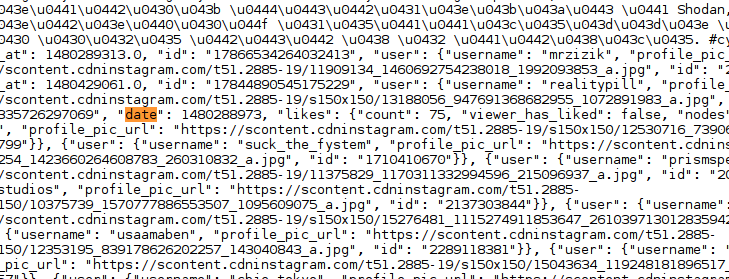
\includegraphics[width=120mm]{images/instagram/1.png}
	}
\end{figure}

It means, that I can simply get all data from specific web page even without any authorization. For parsing I used xpath and re library from python. 

\begin{lstlisting}
script = html.xpath('//script[contains(., "window._sharedData")]/text()')[0]
data = re.search(r"window._sharedData = (.*?);\$", script).group(1)
data = json.loads(data)
\end{lstlisting}

All data was stored in \textbf{data} array.

\subsection{Finding range of instagram ip}

We ask to give us all university netflow traffic for analyzing, it is stored on our computers. The difference of Instagram in comparison with other social network, is that Instagram has very narrow area of usage. In this network users can only add and comment their photos. Every user’s action connected with photos. It means, that instagram need less computer capacity, than other networks. And also Instagram now belong to facebook. The problem was to find exact range of Instagram ip addresses. 

Instagram hasn’t got it’s own autonomous system, but most number of requests send to 31.13.93.72 or 31.13.92.32 or 31.13.93.54. For the first sight we can assume that we should only restrict 31.13.92.0/24 or 31.13.93.0/24. But that is not a solution, because not every address in this network belongs to Instagram.

So, I deсided to find all Instagram ip addresses by myself. I extract all unique destination ip addresses from netflow traffic and get 106 MB file with 6291215 lines. I write a script to revesre-resolve all ip addresses and find Instagram string in it. It was bad idea. Script worked for three days, but process was not finished. And during this I find another solution for this. I decided to use all 31.13.0.0/16 network, and resolve Instagram ip addresses after it.

\subsection{Extracting data from netflow}

In my script I used only raw nfdump. You can see the whole string filter bellow:

\begin{lstlisting}
\$ nfdump -R /var/flows/MYROUTER "dst net 31.13.0.0/16 and port 443" -o csv -t 2016/11/27.22:47:26-2016/11/27.22:47:56 -s record/bytes | head -n -3 | sed '1d'
\end{lstlisting}

The result of such execution:

\begin{lstlisting}
('2016-11-29 15:57:36', '10.240.20.237', '31.13.72.53', '40166', '255667')
('2016-11-29 15:57:22', '10.91.35.114', '31.13.72.8', '57339', '15368')
('2016-11-29 15:57:24', '10.240.20.133', '31.13.92.11', '45988', '8917')
('2016-11-29 15:57:47', '10.240.16.55', '31.13.92.51', '54943', '8843')
('2016-11-29 15:57:35', '10.240.18.181', '31.13.72.53', '62515', '6779')
('2016-11-29 15:57:33', '10.240.16.208', '31.13.72.53', '37487', '5127')
('2016-11-29 15:57:28', '10.242.1.233', '31.13.72.12', '38472', '5122')
\end{lstlisting}

After filtering only Instagram ip addresses it became:

\begin{lstlisting}
('2016-11-29 15:57:36', '10.240.20.237', '31.13.72.53', '40166', '255667')
('2016-11-29 15:57:47', '10.240.16.55', '31.13.92.51', '54943', '8843')
('2016-11-29 15:57:35', '10.240.18.181', '31.13.72.53', '62515', '6779')
('2016-11-29 15:57:33', '10.240.16.208', '31.13.72.53', '37487', '5127')
\end{lstlisting}

The main thing, that I should solve is to find necessary time range. At the moment when user post photo to his Instagram account, long tcp connection should occur, so this connection can start early or end later, that exact post time. With empirical analysis I detect that I should take 20 seconds offset before exact time post and 10 sec offset after timepost. This range give valid results.

\subsection{Experimental results}
In my part of project I trying to map internal ip address on company network to the post in Instagram. To accomplish this I should take time range in 30 seconds, with 20 seconds offset between exect post time and 10 seconds offset after post time. You can see the whole log of program bellow:

\begin{lstlisting}
\$ bin/python netflow.py 
URL to analyze: https://www.instagram.com/p/BNZRbaVgTbv
The post was created at 2016/11/29.12:57:40 GMT
Getting the timerange from netflow dumps: before offset = 20 after offset = 10 GMT offset of netflow server = 3
nfdump -R /var/flows/MYROUTER "dst net 31.13.0.0/16 and port 443" -o csv -t 2016/11/29.15:57:20-2016/11/29.15:57:50 -s record/bytes | head -n -3 | sed '1d'

 At this period of time the following IP addresses was going to instagram website: 

('2016-11-29 15:57:36', '10.240.20.237', '31.13.72.53', '40166', '255667')
('2016-11-29 15:57:47', '10.240.16.55', '31.13.92.51', '54943', '8843')
('2016-11-29 15:57:35', '10.240.18.181', '31.13.72.53', '62515', '6779')
('2016-11-29 15:57:33', '10.240.16.208', '31.13.72.53', '37487', '5127')
('2016-11-29 15:57:34', '10.240.16.157', '31.13.93.52', '53044', '4568')
('2016-11-29 15:57:27', '10.91.42.54', '31.13.92.51', '59556', '4269')
('2016-11-29 15:57:30', '10.240.23.33', '31.13.92.51', '60524', '4019')

 But only following ip addresses get enough bytes from the website: 

('2016-11-29 15:57:36', '10.240.20.237', '31.13.72.53', '40166', '255667')

\end{lstlisting}
